\section{Opto}
The element \(OK_1\) in Figure 13.1 is an optocoupler, which includes a light-emitting diode
(LED) and a photodiode. The photodiode's conductivity depends on the intensity of the
light emitted by the LED, and of course, depends on the current intensity through the
LED. When the voltage across the LED is lower than its barrier potential, the Opto is cutoff. When there is current through the LED, the Opto is in the transfer mode. Like the
current gain \(\beta\) of a BJT, the Opto also has the current transfer ratio (CTR). Assume the LED
has its own barrier potential \(V_F = 1.7\)V, and the Opto has the CTR = 2. Calculate the voltage
\(V_{OUT}\) when the switch is closed. Finally, give your idea about what we may use an Opto
for, and how to use it?

\begin{figure}[ht]
    \centering
    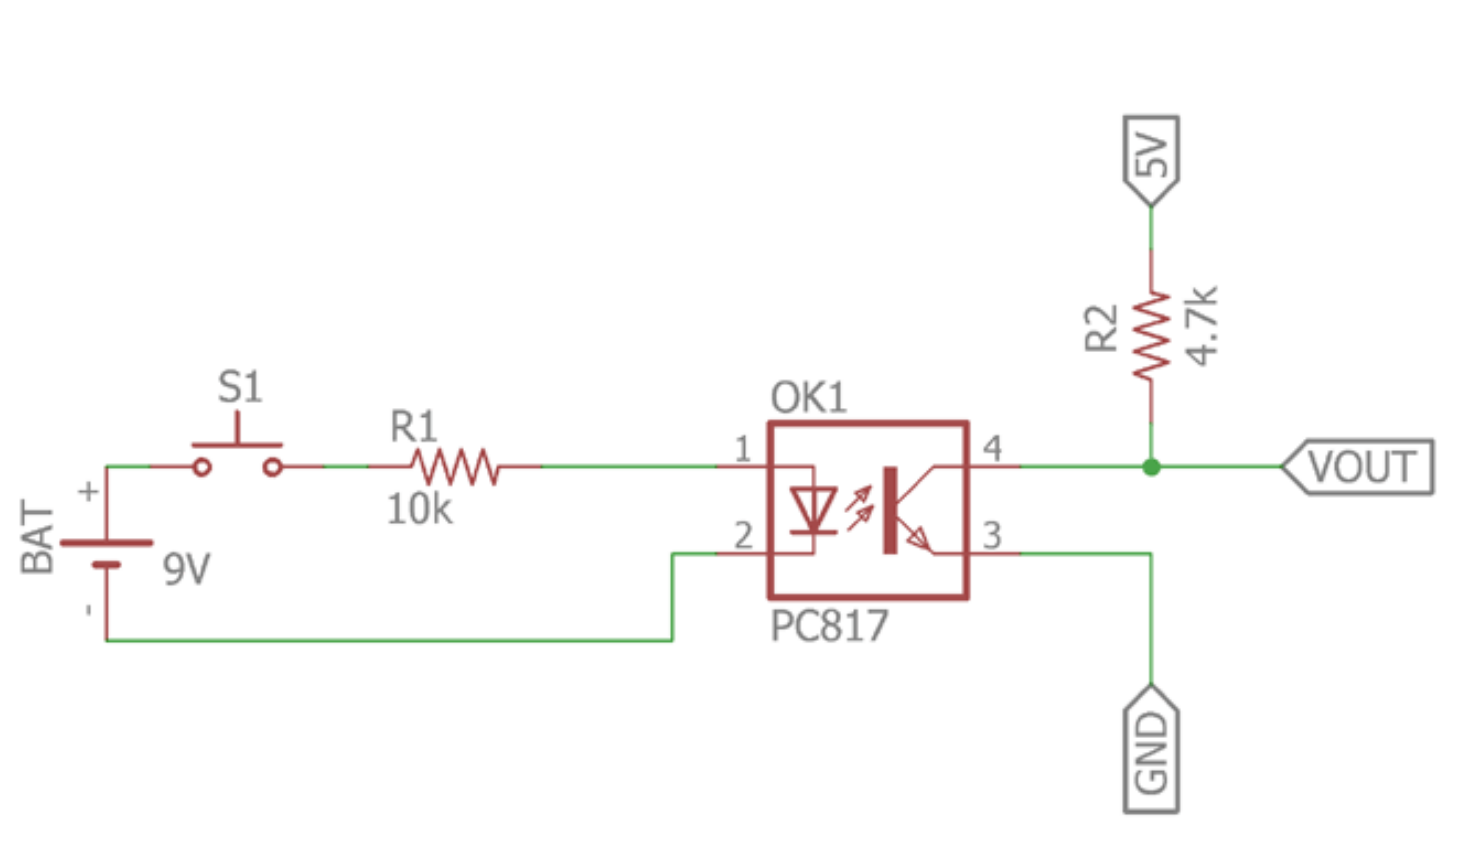
\includegraphics[scale=0.3]{graphics/ex13/f1.png}
    \caption{Voltage isolation with opto}
\end{figure}

\(I_F = I_{R_1} = \dfrac{V - V_F}{R_1} = \dfrac{9 - 1,7}{10.10^3} = 0,73 \) (mA)

\(I_{R_2} = CTR.I_F = 2.0,73 = 1,46\) (mA)

\(V_{OUT} = 5 - I_{R_2}.R_2 = -1,862\) (V)

Nhờ có opto mà hai mạch được cách ly với nhau bởi bộ cách ly quang học. Điều này rất quan trọng đối với hai mạch có sự chênh lệch điện áp lớn. Ví dụ như bộ chuyển đổi tín hiệu giữa các thiết bị có điện áp cao (công tắc giới hạn) và các mạch logic điện áp thấp. 
Hay bảo vệ và cách ly khi sự cố ở tầng đầu ra như cháy, chập, tăng áp,…thì cũng không làm ảnh hưởng đến tầng điều khiển. Cũng như là cách li nhiễu khi kết nối giữa các mạch thu thập thông tin điện áp cao và các mạch logic điện áp thấp, nơi mà các tín hiệu nhiễu có thể gây ra sự cố hoặc lỗi trong hệ thống.
